\documentclass[t]{beamer}
\usecolortheme[RGB={0,114,197}]{structure} 
\usetheme{Ilmenau} 
\usepackage{tikz}
\usepackage{multicol}

\title{Software-Ontwerp}
\subtitle{Iteratie 2}
\author{Castel D. - Devlieghere J. - Pante S. - Reniers V.}
\institute{KU Leuven}

\begin{document}

\frame{\titlepage} 
\begin{frame}{Inhoud}
\begin{multicols}{2}
\tableofcontents
\end{multicols}
\end{frame}



\section{Inleiding} 

\subsection{Rolverdeling}
\begin{frame}{Rolverdeling}
\begin{multicols}{2}
\tableofcontents[currentsection]
\end{multicols}
\end{frame}

\begin{frame}{Rolverdeling}
Afgelopen iteratie:
\begin{itemize}
	\item Lead Designer: Jonas Devlieghere
	\item Lead Tester: Stefan Pante
	\item Domain Modeler: Vincent Reniers
\end{itemize}
Komende iteratie:
\begin{itemize}
	\item Lead Designer: Vincent Reniers
	\item Lead Tester: Jonas Devlieghere
	\item Domain Modeler: Dieter Castel
\end{itemize}
\end{frame}

\subsection{Werkverdeling}

\begin{frame}{Werkverdeling}
\begin{center}
Iteratie 3: 18/03/2013 - 12/04/2013
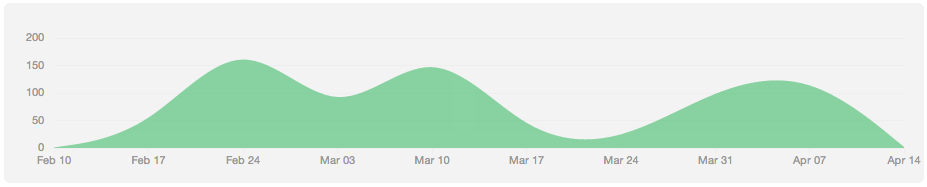
\includegraphics[width= 0.90\linewidth]{images/workload}
\end{center}
\begin{itemize}
	\item Gedurende 8 dagen 6/7 uur per dag
	\item Gemiddeld 50 uur per persoon
\end{itemize}

\end{frame}
\section{Het ontwerp}
\subsection{MVC}

\begin{frame}{MVC}
\begin{center}
%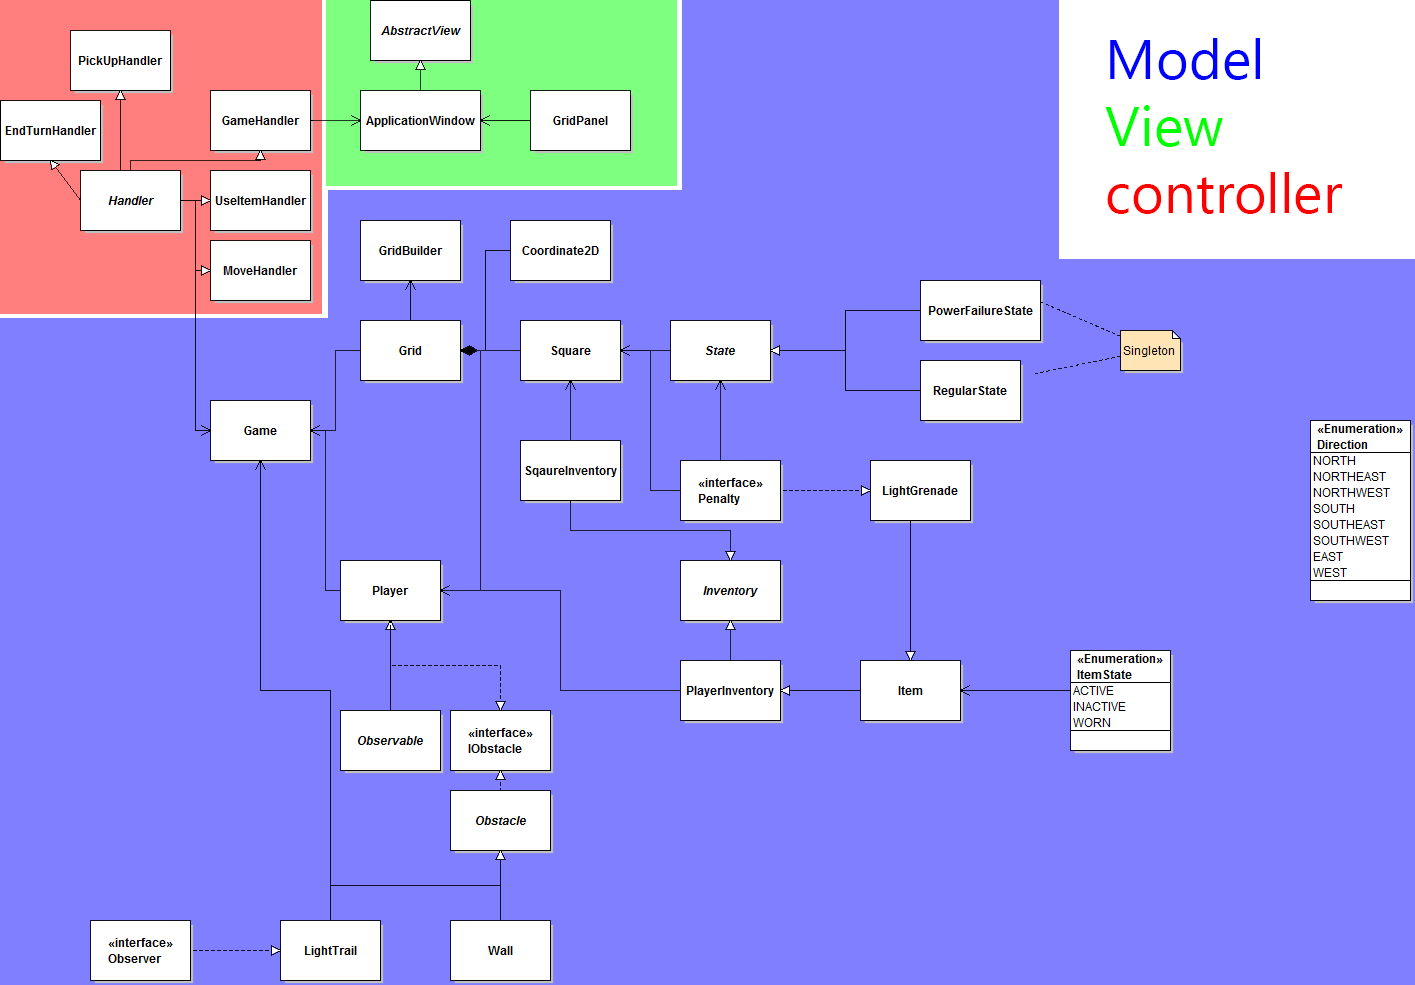
\includegraphics[width=0.9\linewidth]{images/MVC-overview}
\end{center}
\end{frame}

\subsection{Handlers}
\begin{frame}{Handlers}
\begin{center}
%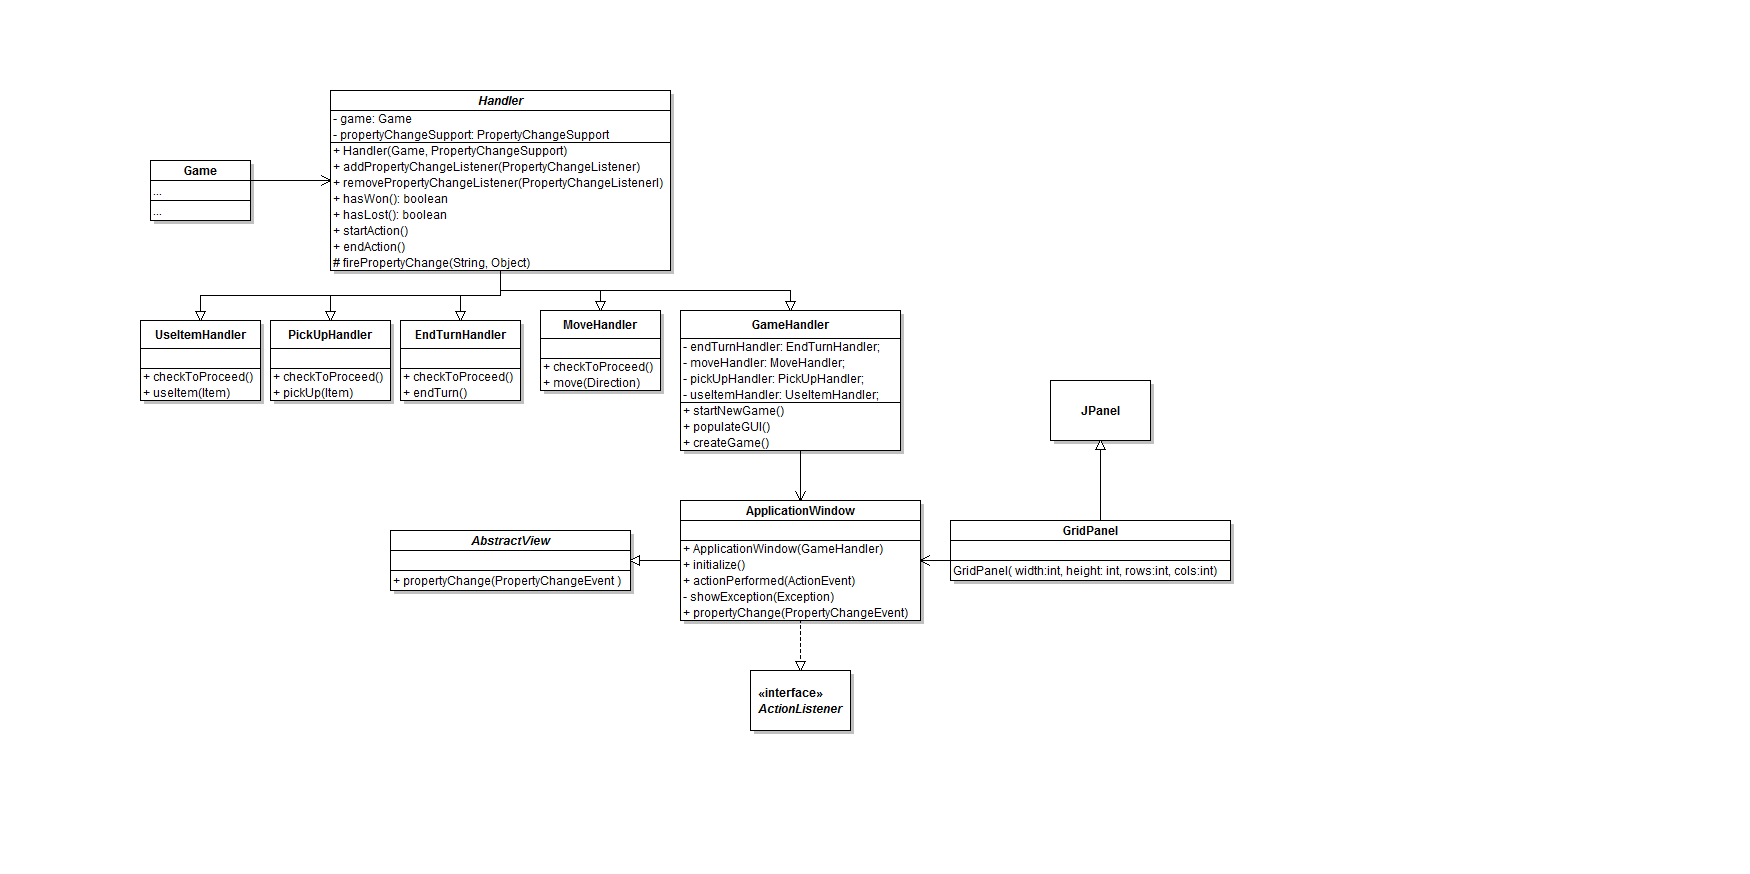
\includegraphics[width=\linewidth]{images/Handlers-View}
\end{center}
\begin{itemize}
	\item Handlers hadden \textit{te veel} verantwoordelijkheid
	\item Uitbreidbaarheid kwam in het gedrang
	\item Juiste flow werd nergens afgedwongen
\end{itemize}
\end{frame}

\subsection{Events}
\begin{frame}{Events}
Gebeurtenis in het spel met vaste volgorde van uitvoering

\begin{multicols}{2}
\begin{center}
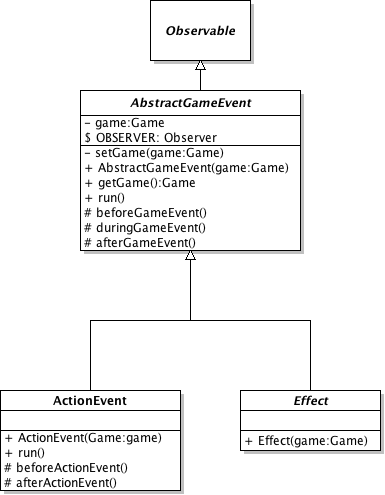
\includegraphics[width=0.60\linewidth]{images/GameEvent}
\end{center}
Flow
\begin{itemize}
	\item \textbf{Voor:} Checks
	\item \textbf{Tijdens:} Eigenlijke afhandeling
	\item \textbf{Na:} Check, gevolgen
\end{itemize}
Twee soorten
\begin{itemize}
	\item ActionEvent
	\item Effect
\end{itemize}
\end{multicols}

\end{frame}

\begin{frame}{ActionEvent}
\begin{itemize}
	\item Gemeenschappelijke checks voor en na de uitvoer
	\item Oberserveerbaar door de TurnHandler
\end{itemize}
\end{frame}

\begin{frame}{ActionEvent}
\begin{center}
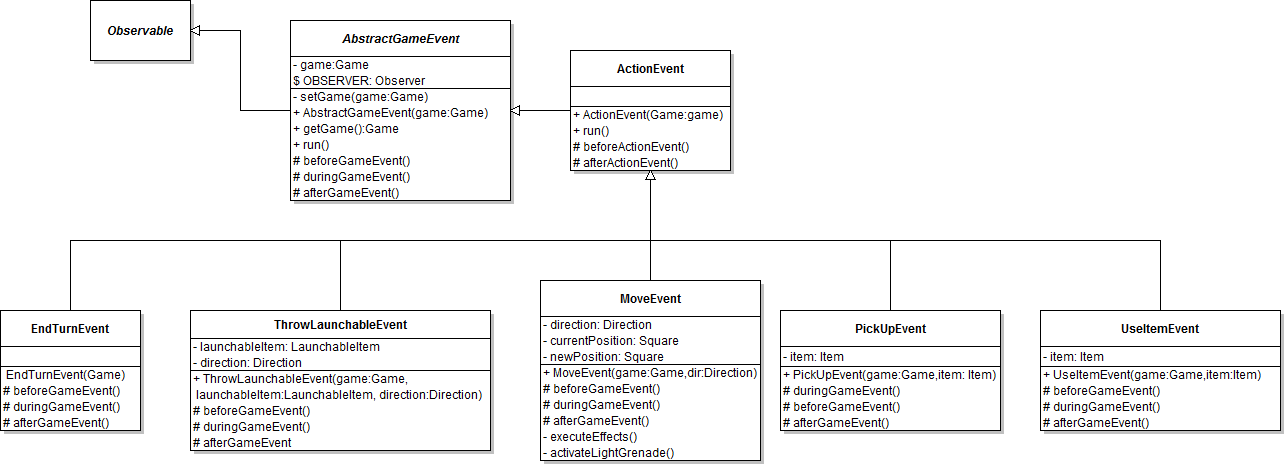
\includegraphics[width=0.65\linewidth]{images/ActionEvents}
\end{center}
\end{frame}

\begin{frame}{Effects}
\begin{center}
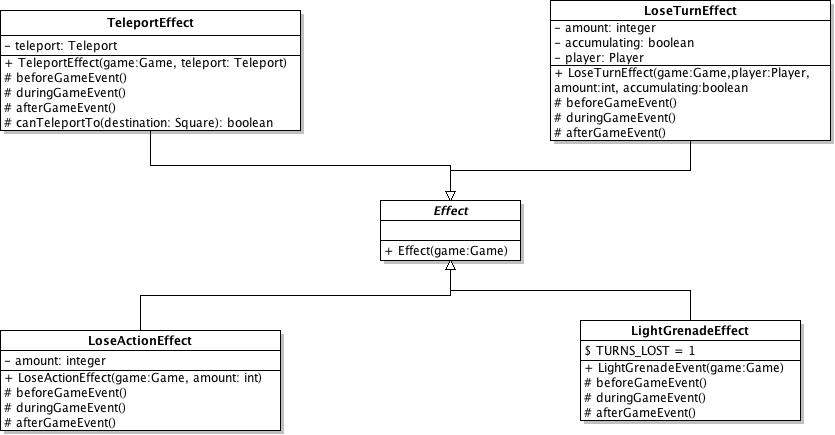
\includegraphics[width=0.75\linewidth]{images/Effects}
\end{center}
\end{frame}

\subsection{Grid}
\begin{frame}{Grid Builder}
\end{frame}

\begin{frame}{Grid Constraint}
\begin{itemize}
	\item \textbf{Percentage:} De limiet op het aantal squares in verhouding met de totale hoeveelheid squares in het grid.
	\item \textbf{Excluded:} Een lijst van squares die niet gekozen mogen worden.
	\item 
\end{itemize}
\end{frame}

\subsection{Obstacles}
\begin{frame}{Obstacle}
\begin{center}
\begin{itemize}
	\item Interface \textit{IObstacle}
	\item  Abstracte klasse \textit{Obstacle} implementeert \textit{IObstacle}
	\begin{itemize}
		\item \textit{LightTrail} implementeert \textit{Obstacle}
		\item \textit{Wall} implementeert \textit{Obstacle}
	\end{itemize}
	\item \textit{Player} implementeert \textit{IObstacle}
	\item \textit{Square} kan \textit{Obstacle} bevatten
\end{itemize}
LightTrail implementeert de \textit{Observer} interface.
\end{center}
\end{frame}


\begin{frame}{Obstacle}
\begin{center}
%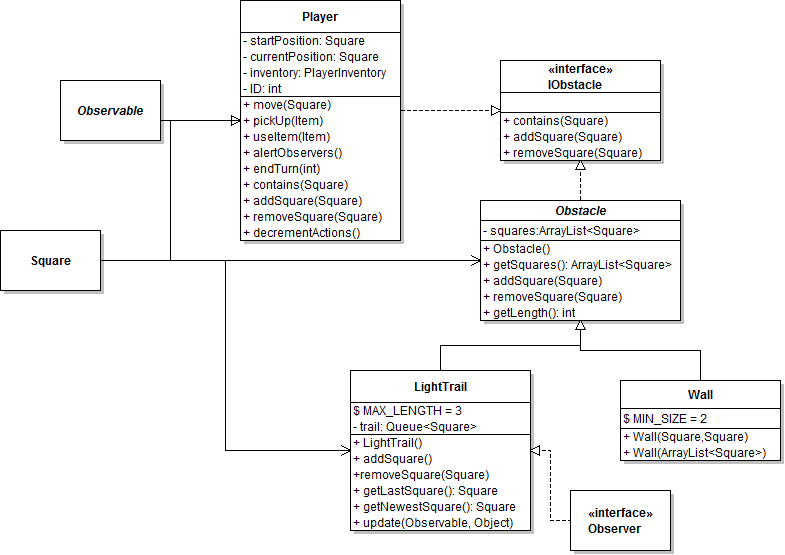
\includegraphics[width=0.70\linewidth]{images/obstacleObserverClassDiagram}
\end{center}
\end{frame}

\subsection{States and Penalty}

\begin{frame}{States and Penalty}
\begin{itemize}
	\item State Pattern
	\begin{itemize}
		\item Square heeft meerdere toestanden: \textit{RegularState}, \textit{PowerFailureState}
		\item Square zorgt voor overgang van staat
	\end{itemize}
	\item Chain of Responsibility (Command)
	\begin{itemize}
		\item State bepaalt eigen penalty
		\item LightGrenade bepaalt eigen penalty
		\item Square is eigenaar van concept penalty
	\end{itemize}
\end{itemize}
\end{frame}

\begin{frame}{States and Penalty}
\begin{center}
%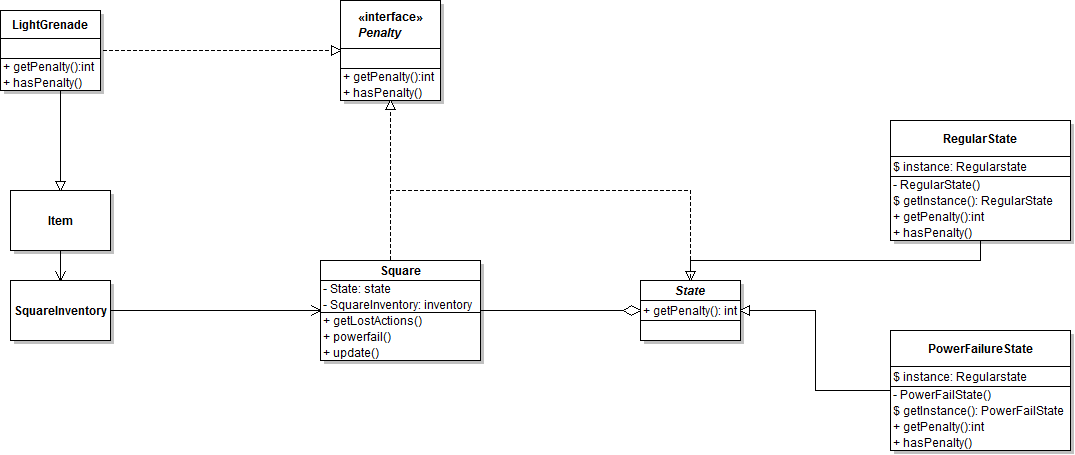
\includegraphics[width=0.90\linewidth]{images/classDiagramStateAndPanelty}
\end{center}
\end{frame}


\section{System State Diagrams}
\subsection{Start New Game}
\begin{frame}{Start New Game}
\begin{center}
%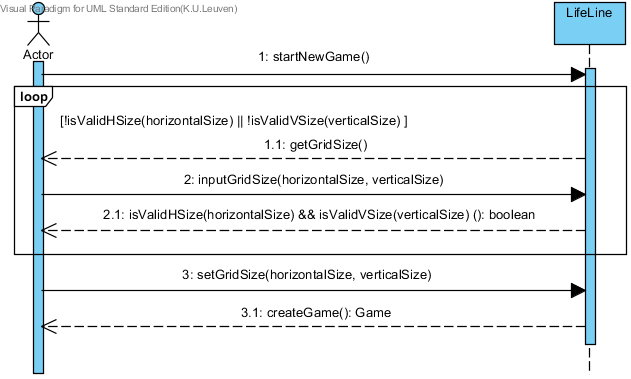
\includegraphics[width=0.90\linewidth]{images/SSDStartNewGame}
\end{center}
\end{frame}

\subsection{Move}
\begin{frame}{Move deel 1}
\begin{center}
%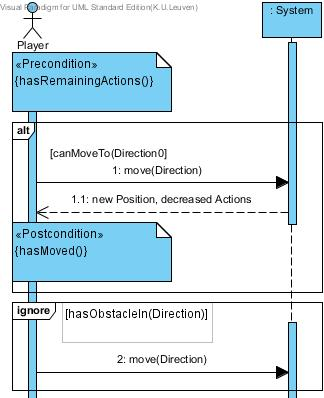
\includegraphics[scale=0.6]{images/SSDMove1}
\end{center}
\end{frame}

\begin{frame}{Move deel 2}
\begin{center}
%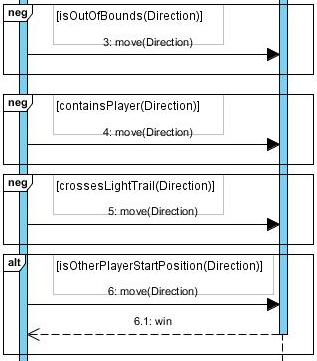
\includegraphics[scale=0.7]{images/SSDMove2}
\end{center}
\end{frame}

\subsection{Pick Up Item}
\begin{frame}{Pick Up Item deel 1}
\begin{center}
%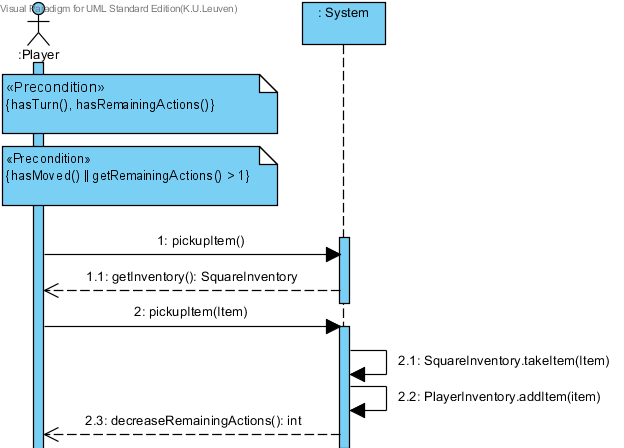
\includegraphics[scale=0.55]{images/SSDPickUpItem1}
\end{center}
\end{frame}

\begin{frame}{Pick Up Item deel 2}
\begin{center}
%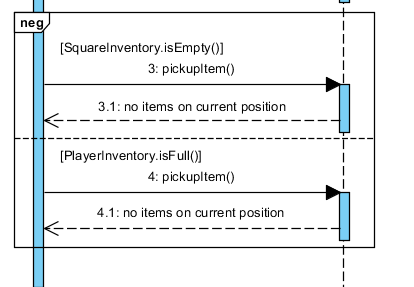
\includegraphics[scale=0.9]{images/SSDPickUpItem2}
\end{center}
\end{frame}


\subsection{Use Item}
\begin{frame}{Use Item deel 1}
\begin{center}
%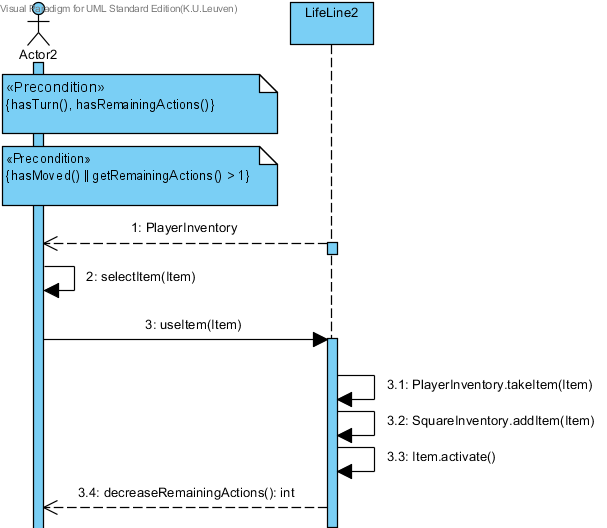
\includegraphics[scale=0.5]{images/SSDUseItem1}
\end{center}
\end{frame}

\begin{frame}{Use Item deel 2}
\begin{center}
%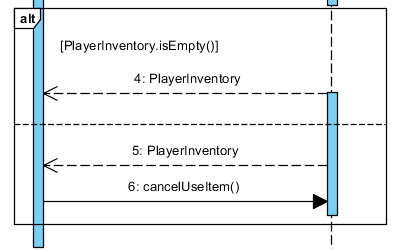
\includegraphics[scale=0.9]{images/SSDUseItem2}
\end{center}
\end{frame}

\subsection{End Turn}
\begin{frame}{End Turn deel 1}
\begin{center}
%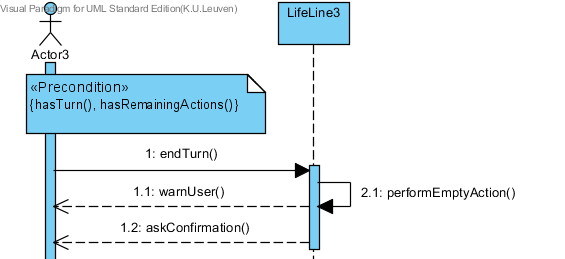
\includegraphics[scale=0.8]{images/SSDEndTurn1}
\end{center}
\end{frame}

\begin{frame}{End Turn deel 2}
\begin{center}
%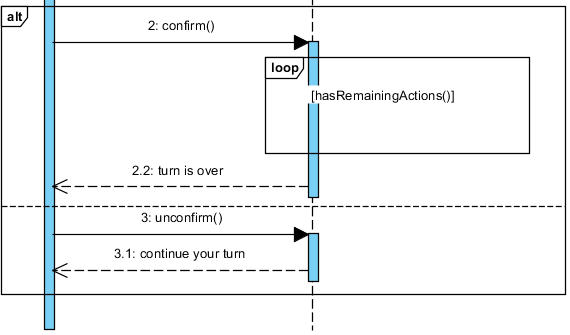
\includegraphics[scale=0.7]{images/SSDEndTurn2}
\end{center}
\end{frame}


\section{Slot}
\begin{frame}{Besluit}
\vspace{0.8in}
\begin{center}
Bedankt voor uw aandacht.
\end{center}
\end{frame}

\end{document}
